% Metaphor: branching tree. One thing divides into cases, and no case
% rejoins another -- reach for it for a taxonomy or a decision. If two
% branches meet again further down, this is not a tree and drawing it as
% one will hide the join.
%
% Idiom: `tree`, via `child`. `level distance` and `sibling distance`
% place every node, so adding a branch re-spaces its whole level instead
% of landing on a neighbour, and the source's own indentation is the
% structure rather than a comment about it.
%
% One thing this idiom costs, worth knowing before you confirm the
% figure: `child` draws its edges internally rather than as `\draw`, so
% `python -m chitragupta.review figure` reports no edge list for this
% picture at all. That is the aid being silently short, not the figure
% being unwired -- read the nesting below for what connects to what.
% House palette (docs/TIKZ-STYLE.md). These five lines travel *inside*
% every figure that uses them -- not a shared file, not a preamble: the
% renderer injects only \usepackage{tikz}, and a thesis fragment is
% \input into a document that has never heard of this project.
\definecolor{cgInk}{HTML}{1A1A1A}
\definecolor{cgFlow}{HTML}{0072B2}
\definecolor{cgAccent}{HTML}{D55E00}
\definecolor{cgAlt}{HTML}{009E73}
\definecolor{cgAux}{HTML}{56B4E9}
\usetikzlibrary{trees}
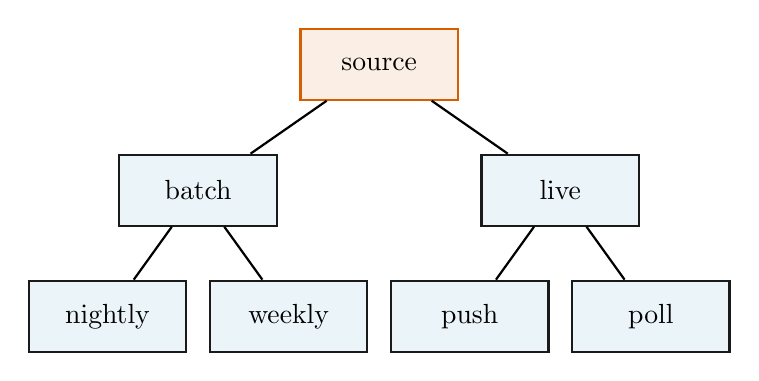
\begin{tikzpicture}[thick,
                    level distance=16mm,
                    level 1/.style={sibling distance=46mm},
                    level 2/.style={sibling distance=23mm},
                    every node/.style={draw=cgInk,align=center,fill=cgFlow!8,
                                       minimum width=20mm,minimum height=9mm}]
  \node[draw=cgAccent,fill=cgAccent!10] (source) {source}
    child { node (batch) {batch}
      child { node (nightly) {nightly} }
      child { node (weekly) {weekly} } }
    child { node (live) {live}
      child { node (push) {push} }
      child { node (poll) {poll} } };
\end{tikzpicture}
